\documentclass[authoryear]{elsarticle}
\usepackage{latexsym}
%\usepackage{rotate}
\usepackage{graphics}
%\usepackage{amsmath}
\usepackage{comment}
\bibliographystyle{chicago}



\newcommand{\logit}{\mathrm{logit}}
\newcommand{\I}{\mathrm{I}}
\newcommand{\E}{\mathrm{E}}
\newcommand{\p}{\mathrm{P}}
\newcommand{\e}{\mathrm{e}}
\newcommand{\vecm}{\mathrm{vec}}
\newcommand{\kp}{\otimes}
\newcommand{\diag}{\mathrm{diag}}
\newcommand{\cov}{\mathrm{cov}}
\newcommand{\eps}{\epsilon}
\newcommand{\ep}{\varepsilon}
\newcommand{\obdots}{\ddots}    % change this later
\newcommand{\Ex}{{\cal E}}
\newcommand{\rat}{{\frac{c_{ij}}{c_{i,j-1}}}}
\newcommand{\rmu}{m}
\newcommand{\rsig}{\nu}
\newcommand{\fd}{\mu}
\newcommand{\tr}{\mathrm{tr}}
\newcommand{\cor}{\mathrm{cor}}
\newcommand{\bx}[1]{\ensuremath{\overline{#1}|}}
\newcommand{\an}[1]{\ensuremath{a_{\bx{#1}}}}

\newcommand{\bi}{\begin{itemize}}
\newcommand{\ei}{\end{itemize}}
\newcommand{\be}{\begin{equation}}
\newcommand{\ee}{\end{equation}}
\renewcommand{\i}{\item}
\newcommand{\sr}{\ensuremath{\mathrm{SRISK}}}
\newcommand{\cs}{\ensuremath{\mathrm{CS}}}
\newcommand{\cri}{\ensuremath{\mathrm{Crisis}}}
\newcommand{\var}{\ensuremath{\mathrm{VaR}}}
\newcommand{\covar}{\ensuremath{\mathrm{CoVaR}}}
\newcommand{\med}{\ensuremath{\mathrm{m}}}
\newcommand{\de}{\mathrm{d}}
\renewcommand{\v}{\ensuremath{\mathrm{v}_q}}
\newcommand{\m}{\ensuremath{\mathrm{m}}}
\newcommand{\tvar}{\ensuremath{\mathrm{TVaR}}}



\newcommand{\eref}[1]{(\ref{#1})}
\newcommand{\fref}[1]{Figure \ref{#1}}
\newcommand{\sref}[1]{\S\ref{#1}}
\newcommand{\tref}[1]{Table \ref{#1}}
\newcommand{\aref}[1]{Appendix \ref{#1}}




\newcommand{\cq}{\ , \qquad}
\renewcommand{\P}{\mathrm{P}}
\newcommand{\Q}{\mathrm{Q}}





\begin{document}

% Title of paper
\title{Systemic risk and contagion effects in Australian financial institutions and sectors}
% List of authors, with corresponding author marked by asterisk
\author{Piet de Jong,  Geoff Loudon and Weihao Choo \\[4pt]
% Author addresses
\textit{Department of Applied Finance and Actuarial Studies\\ Macquarie University, Sydney, NSW 2109.}
\\[2pt]
%E-mail address for correspondence
{piet.dejong@mq.edu.au}}

% Running headers of paper:
\markboth%
% First field is the short list of authors
{De Jong}
% Second field is the short title of the paper
{Systemic risk}

\maketitle

\section{Literature review}

The starting point for the proposed research is the recent literature and the CIFR targeted areas and APRA aims and functions.
This recent literature includes the following
\cite{adrian2011covar},
\cite{acharya2012capital},
\cite{acharya2012measuring}
and \cite{brownlees2010volatility}.   The proposed research aims to extend and apply these techniques particularly in relation to the entities regulated by APRA.   Thus our  broad aim is to develop, implement and bring to bear recent developments in stress testing  on the aims of APRA and the CIFR targeted research areas detailed above.   

\section{Improved  measures of contagion and systematic risk}
\renewcommand{\c}{\ensuremath{\mathrm{CoVaR_q}}}
\renewcommand{\v}{\ensuremath{\mathrm{VaR}_q}}

$\covar_q$ as proposed in \cite{adrian2011covar} is a basis for proposed measures contagion, exposure and systemic risk.   It  suffers from a number of drawbacks:
\bi
\i Couched in terms of $\var_q$ containing the scale of the original measurements.   It is worthwhile to have measures and techniques robust to scale.
\i  Conditioning  on $\var_{0.5}$ is undesirable and relatively intractable.  In our proposal we reference stress with respect  to the unconditional $\var_q$.   This permits a more transparent analysis and estimation. 
\i  Our proposed approach  separates out scale effects and interdependence effects and aims to  relates these separately to external variables including shocks and drivers of systemic risk.   Thus $\var_q$ movements due to scale are disentangled from movements due to codependence with separate driver responses.
\ei

\section{Significance of the project and  policy implications}

Understanding the impact of external shocks and their propagation through   the financial system is vital for managing and remediating systemic risk. Effective regulation is dependent upon the development of a robust and reliable set of appropriate risk measures.  We propose new measures of systemic risk that relate marginal and joint distributions separately to external drivers. This allows for more cogent and coherent stress testing as it includes the estimation of contagion effects, exposure effects and systemic risk across related entities and different financial sectors. Improved stress testing, estimation of risk effects and transmission of shocks through the financial system will make for more cogent prudential policy, prudential margin setting and better identify sources of risk to the financial system.

\newcommand{\q}{\mathrm{Q}}
\section{Percentile sensitivity and contagion}\label{perc}

\subsection{Theorem}  Suppose $x$ is a random vector with marginal distributions\footnote{To economise on notation, write $F_j(x)\equiv F_j(x_j)\equiv F(x_j)$ and } 
$$
F(x)\equiv \{F(x_1),\ldots ,F(x_p)\} \equiv (u_1,\ldots,u_p)\equiv u\ .
$$ 
Further suppose $0\le q\le 1$ is given and  $\q(x)$ is the vector of $q$--quantiles
$$
F\{\q(x)\}=q1=\q(u)\ ,
$$
where $1$ is a vector of $p$ ones. 
Define the stress vector with respect to $x_j$ as\footnote{In \cite{adrian2011covar}  $\Delta CoVar_q\equiv q_{y|x=q_x}-q_y$.  Variable $y$  is generally the ``financial system" and hence considered is the change in the \v\ of the system when institution $x$ stressed, with stress  interpreted as $x=q_x$.  On page 10 of their paper they incorrectly state ``... $CoVaR$ conditions on the event that [an] institution is at its VaR level, which occurs with probability $q$."} 
\be\label{stress}
\frac{\de\q(x)}{\de x_j} \equiv \q(x|u_j>q) - \q(x)\ ,
\ee
where $\q(x|u_j>q)$ is the vector of $q$--quantiles of $x$ given $u_j>q$.    Then if $\q(x)$  is linear in $q$ 
 then
\be\label{implicit}
\frac{\de\q(x_i)}{\de\q(x_j)} \equiv \frac{\de\q(x_i)/\de x_j}{\de\q(x_j)/\de x_j} =  
\frac{f_j}{f_i} 
 \frac{q_{ij}}{q(1-q)}\cq q_{ij}=C_{ij}(q+q_{ij},q) - q^2\ ,
\ee
where $f_i$ and $f_j$ are the densities of $x_i$ and $x_j$ evaluated at their $q$--quantiles and  $C_{ij}$ is the copula of $(u_i,u_j)$.   
Further if 
$$
s_{ij}\equiv \frac{q_{ij}}{q(1-q)}\ ,
$$ then  $-1\le s_{ij}\le 1$ with $s_{ij}=\pm 1$ if $x_i$ and $x_j$ are comonotonic and counter monotonic, respectively.  If $x_i$ and $x_j$ are independent then  $s_{ij}=0$. If $u_i$ and $u_j$ are exchangeable  then  $s_{ji}=s_{ij}$.

\subsection{Implementation}

\fref{fig1} displays the empirical copulas calculated from four weekly closing stock prices labelled anz, cba, mcq and  wbc for $n=761$ weeks from 2000 April 12 through to 2014 October 29.  The empirical copulas are calculated by converting each observation to an empirical percentile and plotting the same against each of the other series percentiles.  

\begin{figure}
  \begin{center}
    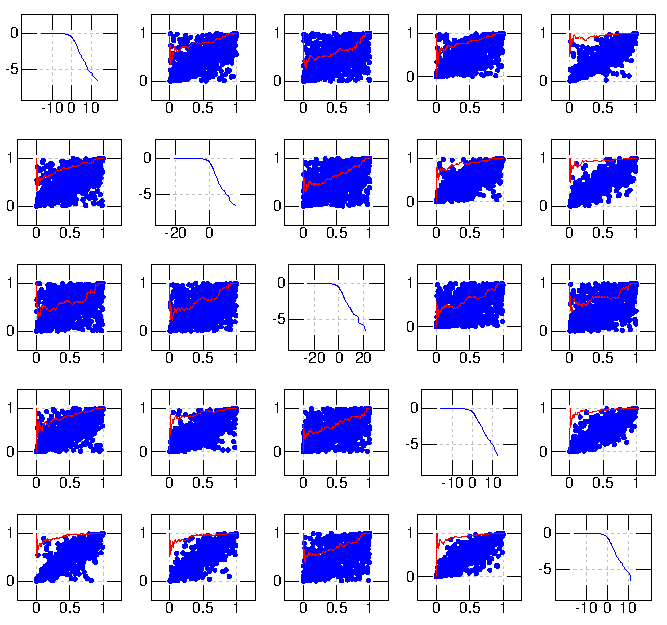
\includegraphics{fig1.pdf}
    \caption{Pairwise copulas of bank stocks  cba, anz, mqg, wbc, and the overall bank index.  Red lines plot sensitivity $s_{ij}$ as a function of $q$.}\label{fig1}
   \end{center}
\end{figure}

To estimate  $q_{ij}$  at a particular $q$, the second equation in \eref{implicit} is iterated\footnote{The second equation in \eref{implicit} is a contraction mapping and hence has a fixed point.} starting from $q_{ij}=0$ where copulas are estimated as 
$$
\hat C_{ij}(u_i,u_j) \equiv \hat\E\{(p_{ik}\le u_i)(p_{jk}\le u_j)\}\ .
$$
Here $\hat\E$ computes the empirical mean over the cases $k=1,\ldots,n$ and $p_{ik}$ and $p_{jk}$ are the empirical percentiles  of case $k$ of $x_i$ and $x_j$, respectively.

\subsection{Discussion}  The critical aspect of the result is that sensitivities factor into contributions from the ratios of the marginal densities and quantities calculated from the pairwise copulas.  The via  the implicit  equation for $q_{ij}$ in \eref{implicit}, solved using a  root finding algorithm.
  The quantities $q_{ij}$ are implicitly defined from the pairwise copulas. In summary 
$$
S \equiv \frac{\de Q(x)}{\de Q'(x)}\ ,
$$
where $'$ denotes transposition.   The matrix $S$ is called the sensitivity matrix and displays the sensitivity of the $q$--quantile of  each component of $x$ to  stress in the same or other components.  Stress in $x_j$ implies that the density of  $x_j$  changes from  $f(x_j)$ to 
$f(x_j)/(1-q)$ where $x_j>\q(x_j)$, called  $q$--stressing $x_j$.  

The ratio of the densities can be written as the ratio of hazards:
$$
\frac{f_j}{f_i} = \frac{\mu_j}{\mu_i}\ ,
$$
since both are evaluated at their respective $q$--quantiles.  This result is useful since the hazard may be better behaved, or easier to model, than the density.

Note that the new density evaluated at $\q(x_j)$ is the hazard at $\q(x_j)$:
$$
\mu_j\equiv \frac{f_j}{1-q}
$$
Hence
$$
\frac{\de\q(x_i)/\mu_i}{\de\q(x_j)/\mu_j}  =  \frac{q_{ij}}{q(1-q)}
$$
\subsection{Proof}

By definition
$$
\frac{\de\q(u_i)}{\de u_j} \equiv \q(u_i|u_j>q) -q \equiv q_{ij}
$$
and  $q_{ij}$ is such that
\be\label{Qdef}
q =  \frac{\P(u_i\le  q+q_{ij},u_j>q)}{1-q}  = \frac{ q+q_{ij}-C_{ij}(q+q_{ij},q)}{1-q}\ ,
\ee
Rearranging yields the second equation in \eref{implicit}.
Now
 \be\label{first}
 \frac{\de\q(x_i)}{\de x_j}\equiv F_i^-(q+q_{ij}) - \q(x_i) \approx (F_i^-)'(q)q_{ij}= \frac{q_{ij}}{f_i} \ ,
 \ee
where $'$ denotes differentiation.  The approximation follows from a first order Taylor expansion and is exact if the quantile is linear in $q$.   Similarly
 \be\label{second}
 \frac{\de\q(x_j)}{\de x_j}\equiv  F_j^-\{q+q(1-q)\} - \q(x_j)\approx \frac{q(1-q)}{f_j}\ .
 \ee
 Dividing \eref{first} by \eref{second} yields the first equation in  \eref{implicit} and completes the proof.
 
 \subsection{Further remarks}
 
 Note that
 $$
 \frac{\de\q(x_i)}{f_j\de x_j} = \frac{\de\q(x_i)}{f\{\q(x_j)\}\de x_j} = \frac{\de\q(x_i)\de\q(x_j)}{\de F\{\q(x_j)\}\de x_j}=\frac{\de\q(x_i)/\de x_j}{\de F\{\q(x_j)\}/\de\q(x_j)}
 $$
 
 Using the usual rules of calculus
 $$
 \frac{\de\q(x_i)}{\de \q(x_j)} = \frac{\de \q(x_i)}{\de u_i} \frac{\de u_i}{\de u_j}\frac{\de u_j}{\de\q(u_j)}= \frac{\de \q(x_i)}{\de u_i} \frac{\de u_i}{\de u_j}\frac{1}{q(1-q)}
 $$
 Now
 $$
 \frac{\de \q(x_i)}{\de u_i} =\frac{F^-(q_i)}{} \cq \frac{u_i}{u_j} = q_{ij} 
 $$
 $$
   \frac{\de\q(x_j)}{\de x_j}= f(x_j)\frac{\de\q(x_j)}{\de u_j}\qquad\Rightarrow \qquad  \frac{\de\q(x_j)}{\de \q(x_i)}
 $$
 $$
  \frac{\de q}{\de u_j} = \frac{\de F\{\q(x_i)\}}{\de u_j} =  f_i\frac{\de\q(x_i)}{\de u_j} \qquad\Rightarrow\qquad 
 $$

\subsection{Generalisations}
Can the above be generalised to other risk measures?   Suppose $\q(x)\equiv\E\{x\phi(u)\}$ where $\phi$ is a given function which acts componentwise and $x\phi(u)$ denotes componentwise multiplication.  Then the analogue of \eref{stress} is 
\be\label{stress2}
\frac{\de\q(x)}{\de x_j} \equiv \q\{x|x_j>\Q_j(x)\} - \q(x)\ ,
\ee
where stress is  $x_j>\q_j(x)$.   In this case we assume $\q(x)$ is again linear when we cut the left tail off (how to formalise exactly -- maybe linearity is more appropriate in other risk measures)     



\begin{comment}

If $\dot q'_{uv}$ is the derivative of $\dot q_u$ with respect to $q$ then
$$
\dot q_{uv}= (1+\dot q_{uv})C_u(q+\Delta_v q_u,q)+C_v(q+\Delta_v q_u,q)-2q
$$
where $C_u$ and $C_v$ are the partial derivatives of $C$ with respect to $u$ and $v$, respectively.
\end{comment}


\section{Financial sensitivity and contagion}
 

The matrix $S$ of sensitivities can be decomposed with the singular value decomposition
$$
S = UDV' = s_1c_1' + s_2c'_2 + \cdots + s_pc_p'\ .
$$
Here  $D$ a diagonal matrix of singular values, arranged in decreasing order along the diagonal.  So the best thing is to compare 
$$
Q= s_{i1}c_{j1} + \cdots + s_{ip}c_{jp} 
$$

If $Q=I$ then $S=C=I$.   If $Q=11'$, a matrix of ones, then $S=\sqrt{p}(1,0)$ and $C=(c,0)$ both have rank 1:  here $s$ and $c$ are the leading columns of $S$ and $C$, respectively and 0 a matrix of zeros.

The approximation $Q\approx sc'$ is exact if $Q$ has rank 1 implying $Q=11'$.   The approximation $Q\approx sc'$ is inadequate if $Q=I$.  Inadequacy can be judged from the largest singular value in $D$, as a proportion of $p$, the number of variables or rows in $Q$.

$$
Q_* \equiv \frac{1}{p-1}(Q-I)=UDV'\cq s\equiv Q_*1\cq c\equiv Q_*'1\ .
$$$$
Q=I + s1'+ UDV'\cq s\equiv \frac{1}{p-1}(Q-I)1
$$
Then $s$ is the vector of average \v\ sensitivity of each variable to all others.  Further $c$ is the average \v\ impact of each variable on all others.   The matrices $U$, $D$ and $V$ define the singular value (svd) decomposition of $Q_*$, arranged so that diagonal matrix $D$ has the singular values on  the diagonal in descending order.   If $b=d_1u_1$ and $c=v_1$ where $u_1$, $d_1$ and $v_1$ are the first column, top diagonal entry, and first column of $U$, $D$ and $V$ respectively, then  for two variables $y\ne x$ in $Q$,
$$
\Delta_x q_y = s_y+ b_yc_x +\eps_{yx}
$$
This states that percentage sensitivities are, apart from the ``error" $\eps_{yx}$, an average sensitivity plus a scaled response to the contagious effect of the $x$ variable.   The contagious effects contained in $c$ are estimated by maximising the explanation of $Q$.


The vector $1'Q$ sums  the changes in \v\ when each of the column variables is stressed, and writes this as a proportion of the change in the variable being stressed.   These proportional sums, subtracting 1 and divided by  $p-1$ where $p$ is the number of variables, measures the average contagion of each variable on all others:  $c'=(p-1)^{-1}1'(Q-I)$ or $c=(p-1)^{-1}(Q-I)'1$

Alternatively the vector $Q1$ sums the changes in \v\ of each row variable when all the column variables are stressed.   Again it is appropriate to remove the effect of a variable on itself and consider the average over the remaining variables:  $s\equiv(p-1)^{-1}(Q-I)1$.  If $Q_*\equiv (p-1)^{-1}(Q-I)$ then $s=Q_*1$ and $c=\dot q_*1$ are the vectors of sensitivities and contagions, respectively.  If $Q=I$ then $s=c=0$.   If $Q=11'$ then $s=c=1$.



 
 \section{Systemic risk and causal chains}
A rank one approximation to the matrix  $Q$ is 
 $
 Q  \approx  sc' 
 $.
 Vector $c$ is an index of the contagious  impact of each of variables on the others while $s$ measures the sensitivity of each variable to each of the others.  The vectors $s$ and $c$ are derived from the singular value decomposition $Q=UDV'$ where $U'U=V'V=1$  and  where $s$ and $c$ are the first column of $UD$ and $V$  respectively, assuming the svd is organised so that the singular values in the diagonal matrix $D$ are organised from largest to smallest.   The appropriateness of the summarisation $sc'$ is measured with $\tr(Q-sc')$.
 
If the variables are independent then $Q=I$ and both $s$ and $c$ equal a column of the identity matrix with $sc'$ a matrix of 0's except in a single diagonal position where it is 1.   Then all but one variable has a contagion effect and only that variable is sensitive to the contagion provided by the  variable.

If the variables are comonotonic then $Q=11'$ and $s=1$ and $c=1$ where 1 denotes a vector of ones.   Thus the rank 1 approximation is exact and each variable is equally contagious and equally sensitive.
 
 Note that 
 $$
 Q^{n} \approx (s'c)^{n-1}sc'=\ ,
 $$
 
 
 If the random variables are independent the $Q-I=0$ and $a=b=k=0$ and there is no error in the first order svd approximation.    If the random variables are comonotonic then $Q=11'$ and $Q-I$ has ones everywhere except on the diagonal where it is zero.   The vector of row means is then $p^{-1}(p-1)1$
 
Systemic risk in the system is measured with $b'k=d_1(u_1'v_1)$.   In the case of comonotonic  random variables $Q=11'$, $a=1$ and $x$, where $p$ is the number of variables,  $d_1=1$. 
 
Furthermore we may define quantities such as
$
u^- \equiv \var_q(v|u\le q)
$
measuring the impact of a non distressed state in $v$.  For brevity we do not dwell on these constructs in this writeup although the ramifications and potential uses of these constructs will be  investigated in the research.

\section{Literature}

We propose a measure for systemic risk: CoVaR, the value at risk (VaR) of financial institutions conditional on other institutions being in distress. We define an institution?s (marginal) contribution to systemic risk as the difference between CoVaR and the financial system?s VaR. From our estimates of CoVaR for characteristic-sorted portfolios of publicly traded financial institutions, we quantify the extent to which characteristics such as leverage, size, and maturity mismatch predict systemic risk contribution. We argue for macro-prudential regulation based on the degree to which such characteristics forecast systemic risk contribution.

\section{Econometric implementation}

The above development sets out our proposed  broad  framework for linking bivariate copulas and marginals to external variables and shocks study the impact of the same on stresses within the system and the contagious effects of crises.   Proposed econometric analysis will implement and extend  \cite{brownlees2010volatility}.

\section{Data}

We will employ publicly available data as published by APRA and other regulators.

\section*{References}
\bibliography{/Applications/Tex/piet2}


\end{document}
